%%% Local Variables:
%%% mode: latex
%%% TeX-master: "../demo3"
%%% End:

\setlength{\baselineskip}{16pt}
\chapter{附录~E}\label{appen.e}

\renewcommand{\thetable}{E-\arabic{table}}
\renewcommand{\thefigure}{E-\arabic{figure}}
\renewcommand{\theequation}{E-\arabic{equation}}
\renewcommand{\theHtable}{E.\arabic{table}}
\renewcommand{\theHfigure}{E.\arabic{figure}}
\renewcommand{\theHequation}{E.\arabic{equation}}
\setcounter{table}{0}
\setcounter{figure}{0}
\setcounter{equation}{0}

\begin{center}
\zihao{3}
\textbf{推广策略分区构建}
\end{center}

本附录说明第~\ref{chap.optimization}章中推广策略分区的构建方法。分区的目的是在保留空间异质性的同时，将分区数量控制在代理训练与反向求解可接受的范围内。同一策略分区内的调查智能体在同一阶段接受相同的营销、定价、套餐额度和服务水平决策，不同策略分区之间则允许采用不同策略。北京市16个有效的行政区分区的具体流程如下所述：

\textbf{（1）区级特征构造与归一化}

考虑到推广策略通过影响居民的出行方式选择而间接影响推广效果，因此分区特征变量主要考虑居民的家庭社会经济情况和日常出行方式。为此，对每个行政区构造家庭收入指示变量、家庭是否拥有小汽车、是否为高频公共交通使用者（单日使用超2次）和是否为高频出租车使用者（单日使用超2次）组成的六维特征，以表征各行政区的家庭社会经济结构和出行方式偏好。记行政区$d$的区级特征向量为
\begin{equation}
\bm{x}_{d}
=
\left[
\bar I_{d,1},\,
\bar I_{d,2},\,
\bar I_{d,3},\,
\bar C_{d},\,
\bar P_{d},\,
\bar T_{d}
\right]^{\top},
\label{eq.append.zone.feature}
\end{equation}
式中，$\bar I_{d,1}$、$\bar I_{d,2}$和$\bar I_{d,3}$分别为分区$d$内低、中、高三类收入指示变量的比例，用于描述行政区内家庭收入结构；$\bar C_d$为家庭拥有小汽车的比例；$\bar P_d$为高频公共交通使用者比例；$\bar T_d$为高频出租车使用者比例。

随后，将各区特征拼接为16个区级特征向量，形成96维条件向量
\begin{equation}
\bm{c}
=\mathrm{vec}
\left(
[\bm{x}_{0},\bm{x}_{1},\ldots,\bm{x}_{15}]^{\top}
\right),
\qquad
\tilde{\bm{c}}
=
\frac{\bm{c}-c_{\min}\bm{1}}
{c_{\max}-c_{\min}},
\label{eq.append.zone.scale}
\end{equation}
式中，$c_{\min}$和$c_{\max}$分别为整个96维向量的最小值和最大值；$\bm{1}$为与$\bm c$维度相同的全1向量；$\tilde{\bm c}$为归一化后的条件向量。随后将$\tilde{\bm c}$恢复为$16\times6$的特征矩阵。

\textbf{（2）策略分区聚类}

在上述分区特征向量上，采用K均值聚类对各行政区进行聚类。记$z_d\in\{0,1,\ldots,Z-1\}$为区级编码$d$所属的策略分区，$\bm\mu_z$为分区$z$的聚类中心，则聚类目标为
\begin{equation}
\underset{\{z_d\},\{\bm\mu_z\}}{\min}
\quad
\sum_{d}
\left\|\tilde{\bm{x}}_d-\bm\mu_{z_d}\right\|_2^2,
\label{eq.append.zone.kmeans}
\end{equation}
式中，$\tilde{\bm{x}}_d$为归一化后的六维区级特征。

采用轮廓系数、肘部法等统计准则比较不同聚类数策略分区数，结果如图\ref{fig.Kmeans}所示。综合考虑聚类的轮廓系数、肘部法拐点、策略分区数量与代理模型反向求解可行性，选取$Z=5$为最终聚类数。

\begin{figure}[H]
  \centering
  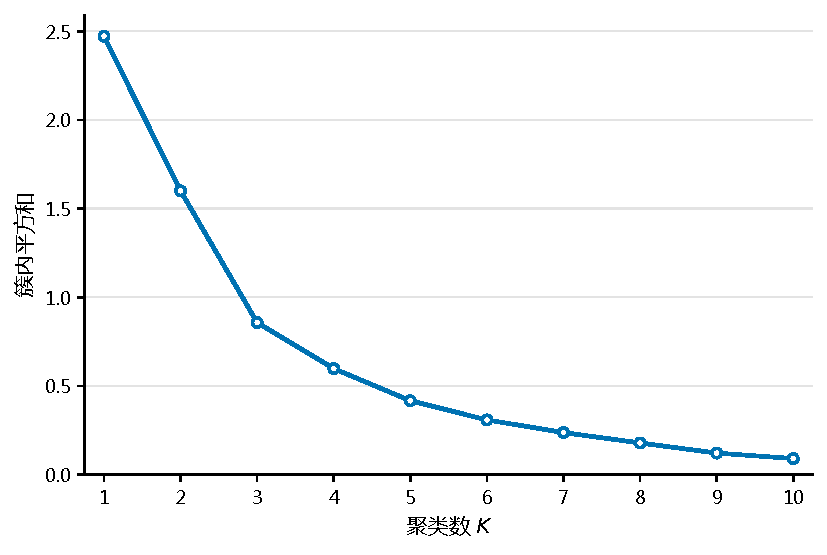
\includegraphics[width=\textwidth]{figures/appendixE/zone_clustering_elbow.pdf}
  \bicaption{K均值聚类轮廓系数变化}{Variation in the silhouette coefficient for K-means clustering.} 
  \label{fig.Kmeans}
\end{figure}

\textbf{（3）策略分区结果}

表~\ref{tab.append.zone.mapping}给出各行政区的调查居民数及其聚类后的策略分区。

\clearpage
{
\small
\setlength{\tabcolsep}{6pt}
\begin{longtable}{C{1.3cm}L{3.6cm}R{3.0cm}C{2.0cm}}
\bicaption{调查区级编码与策略分区映射}{Mapping from survey district codes to promotion strategy zones.}\label{tab.append.zone.mapping} \\
\toprule
序号 & 行政区 & 调查居民数 & 策略分区 \\
\midrule
\endfirsthead
\multicolumn{4}{l}{\small（续表~\ref{tab.append.zone.mapping}）}\\
\toprule
序号 & 行政区 & 调查居民数 & 策略分区 \\
\midrule
\endhead
\midrule
\multicolumn{4}{r}{\small 续下页}\\
\endfoot
\bottomrule
\endlastfoot
1  & 东城区               & 5\,312  & 3 \\
2  & 西城区               & 5\,040  & 0 \\
3  & 朝阳区               & 11\,285 & 0 \\
4  & 丰台区               & 8\,916  & 4 \\
5  & 石景山区             & 4\,229  & 3 \\
6  & 海淀区               & 11\,419 & 0 \\
7  & 房山区               & 3\,375  & 4 \\
8  & 通州区               & 8\,998  & 0 \\
9  & 顺义区               & 3\,910  & 0 \\
10 & 昌平区               & 4\,767  & 0 \\
11 & 大兴区               & 4\,794  & 4 \\
12 & 门头沟区             & 1\,949  & 4 \\
13 & 怀柔区               & 1\,198  & 2 \\
14 & 平谷区               & 1\,286  & 3 \\
15 & 密云区               & 1\,396  & 2 \\
16 & 延庆区               & 1\,354  & 1 \\
\end{longtable}
}
